\subsection{Reference Frames and Transformations}
\subsubsection{Basic Translation and Rotation Transformations}
Rigid body motion in three dimensions can be expressed compactly using the homogeneous transformation matrix $T \in \mathrm{SE}(3)$ defined in Equation \ref{eq:SE3-definition}. These matrices combine rotation and translation into a single representation and are used to map coordinates between frames such as the navigation (NED), body, and sensor frames.  
\\ \\
The pose of the body frame relative to the navigation frame is written as
$$
    T_{b}^{n} =
    \begin{bmatrix}
        R_{b}^{n} & \mathbf{p}_{b}^{n} \\
        0 & 1
    \end{bmatrix}
$$
where $R_{b}^{n}$ is the rotation matrix from the body to the NED frame, and $\mathbf{p}_{b}^{n}$ is the position of the body origin expressed in NED coordinates.
\\ \\
A point $\mathbf{x}_{b}^{b}$ expressed in the body frame can be transformed to the NED frame as:
$$
    \mathbf{x}_{b}^{n}=
    T_{b}^{n}
    \begin{bmatrix}
        \mathbf{x}_{b}^{b} \\ 1
    \end{bmatrix}
    = R_{b}^{n}\mathbf{x}_{b}^{b} + \mathbf{p}_{b}^{n}
$$
\noindent
Composing multiple transformations is performed through matrix multiplication. For instance, if $T_{s}^{b}$ defines the transformation from a sensor frame to the body frame, then the sensor pose in the NED frame becomes
$$
    T_{s}^{n} = T_{b}^{n} T_{s}^{b}
$$
The inverse transformation, which converts coordinates from NED back to the body frame, is given by
$$
    T_{n}^{b} = (T_{b}^{n})^{-1} =
    \begin{bmatrix}
        (R_{b}^{n})^T & -(R_{b}^{n})^T \mathbf{p}_{b}^{n} \\
        0 & 1
    \end{bmatrix}
$$
This matrix formulation provides a clean and consistent way to represent spatial relationships between the navigation, body, and sensor frames. It is fundamental in robotics, navigation, and control, where accurate frame alignment and transformation chaining are essential for pose estimation and sensor fusion.
\\ \\
These homogeneous transformations form the foundation for defining global and local reference frames such as WGS84, ECEF, NED, and Body, which are described in the following sections



\subsubsection{Global Reference Frames}
Global reference frames provide the foundation for representing absolute positions on Earth and are essential for all GNSS based navigation and mapping systems. Since GNSS receivers provide position estimates in a global Earth fixed frame, while navigation and control systems typically operate in local frames such as NED or body coordinates, it becomes necessary to define consistent global reference models to enable accurate transformations between these coordinate systems.   
\\ \\
The two main reference systems used for this purpose are the World Geodetic System 1984 (WGS84) geodetic model, which defines the Earths ellipsoidal shape and geodetic coordinates (latitude, longitude, altitude), and the Earth-Centered Earth-Fixed (ECEF) Cartesian frame, which expresses these same positions as 3D Cartesian coordinates centered at the Earths center of mass. These systems provide the common link between GNSS measurements and local navigation frames used in estimation and control.
\\ \\
\textbf{WGS84} 
\\ \noindent
The World Geodetic System 1984 (WGS84) is the global geodetic reference used by all major GNSS systems. It defines an Earth-fixed ellipsoidal model that closely approximates the planets mean shape, accounting for the equatorial bulge caused by rotation. Although regional realizations such as \textit{``ETRS89''} (European Terrestrial Reference System 1989) are used in Europe to reduce tectonic drift, the WGS84 reference remains the standard for GNSS based navigation in Norway and most marine applications, with differences between the two systems being only a few decimeters.
\\ \\
The WGS84 model defines the Earth as an oblate ellipsoid, flattened at the poles and expanded at the equator. It serves as the global geodetic reference for GPS and most modern satellite navigation systems. The ellipsoid parameters are defined as $a = 6378137.0~\text{m}$ and $f = 1/298.257223563$, where $a$ is the semi major axis and $f$ is the flattening factor. The semi minor axis can then be computed as $b = a(1-f)$.  
\\ \\
A position on Earth is defined by three geodetic coordinates. First the latitude $\varphi$, which is the angle between the equatorial plane and the ellipsoid normal. Then the longitude $\lambda$, which is the angle between the Greenwich meridian and the projection of the point onto the equatorial plane. Finally the altitude $h$, which is the height above the ellipsoidal surface. These coordinates describe a points global position and are the standard output format from all GNSS receivers.
\begin{figure}[H]
    \centering
    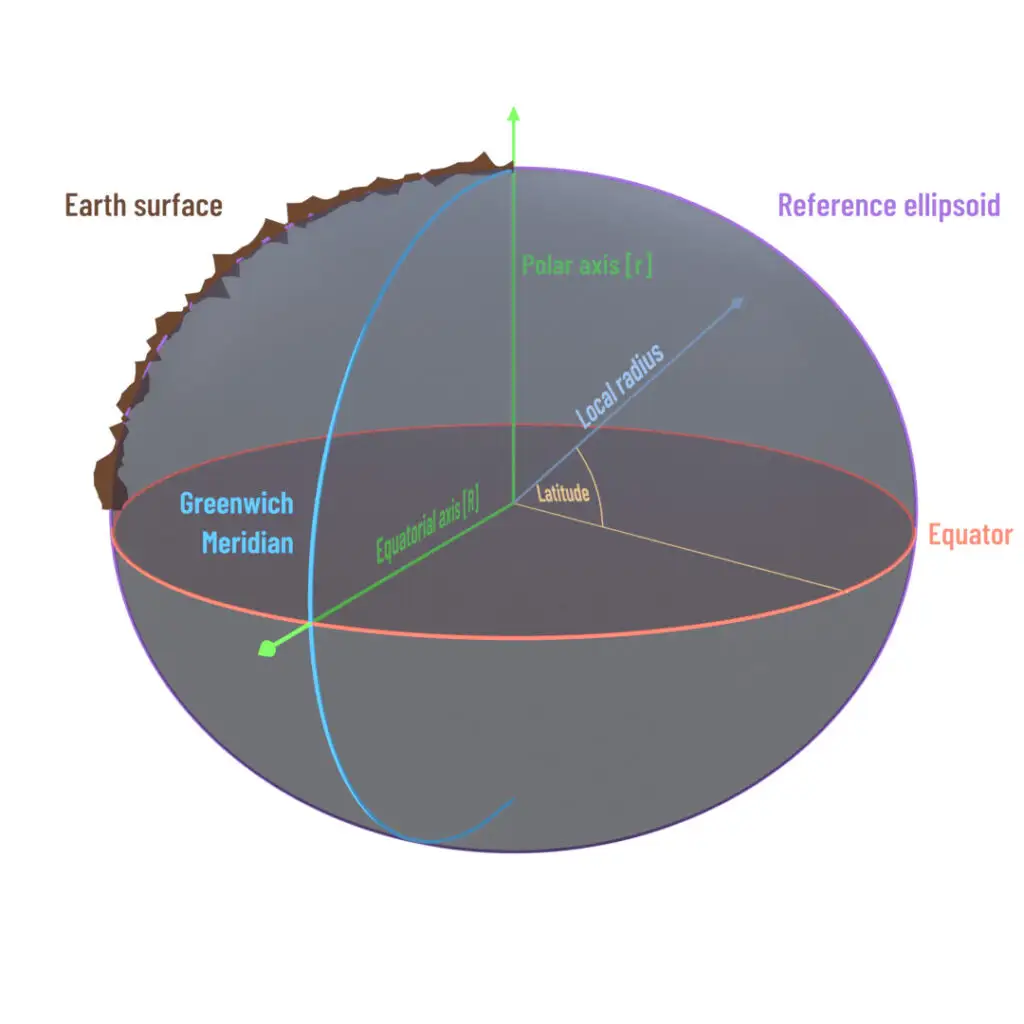
\includegraphics[width=0.7\linewidth]{Pictures/System_Modeling/Reference_Frames_and_Transformations/WGS84.png}
    \caption{WGS84 ellipsoidal Earth model showing the relationship between latitude, longitude, and altitude. Figure taken from GeneSys Elektronik GmbH documentation.\textsuperscript{\cite{WGS84}}}
    \label{fig:system-Modeling-wgs84-ellipsoid}
\end{figure}
\noindent
\textbf{ECEF}
\\ \noindent
The Earth-Centered Earth-Fixed (ECEF) frame is a three dimensional Cartesian coordinate system with its origin at the Earths center of mass. The $x$-axis passes through the intersection of the equator and the Greenwich meridian, the $y$-axis lies along the equator $90^{\circ}$ east of the $x$-axis, and the $z$-axis points toward the North Pole. The ECEF frame rotates with the Earth and is commonly used for expressing GNSS positions in Cartesian form.  
\\ \\
The transformation from geodetic coordinates WGS84 $(\varphi, \lambda, h)$ to ECEF coordinates $(x, y, z)$ is given by:
$$
    \begin{aligned}
        e^2 &= 2f - f^2, \\
        N(\varphi) &= \frac{a}{\sqrt{1 - e^2 \sin^2\varphi}}, \\
        x &= (N(\varphi) + h)\cos\varphi\cos\lambda, \\
        y &= (N(\varphi) + h)\cos\varphi\sin\lambda, \\
        z &= \big[(1 - e^2)N(\varphi) + h\big]\sin\varphi
    \end{aligned}
$$
where $N(\varphi)$ is the prime vertical radius of curvature and $e$ is the first eccentricity of the ellipsoid. The inverse conversion from ECEF to geodetic coordinates is typically solved iteratively due to the nonlinear nature of the equations.
\begin{figure}[H]
    \centering
    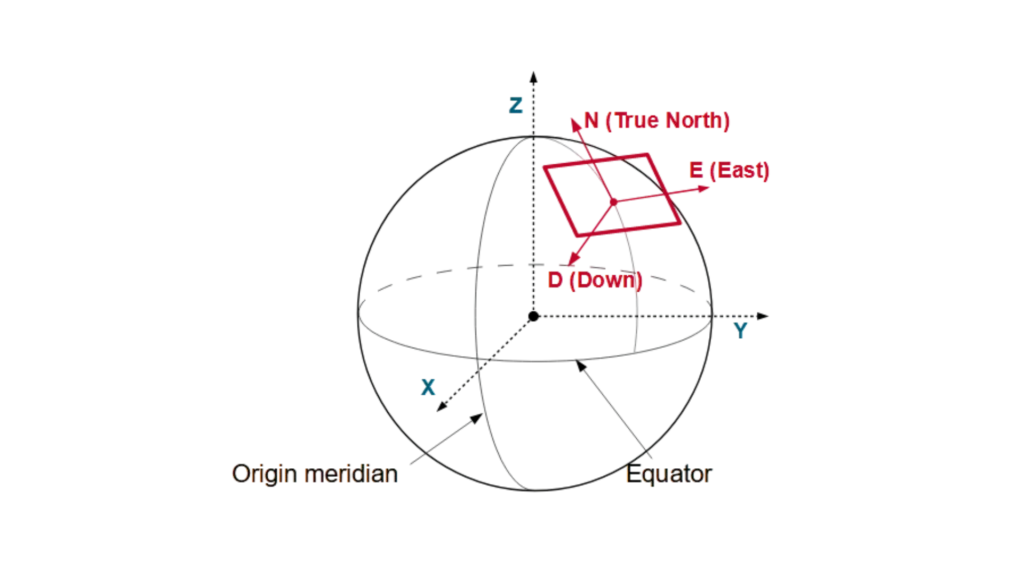
\includegraphics[width=0.9\linewidth]{Pictures/System_Modeling/Reference_Frames_and_Transformations/ECEF.png}
    \caption{Earth-Centered Earth-Fixed (ECEF) coordinate system with origin at Earth's center and axes aligned with the equator and rotational axis. Figure taken from open source GNSS reference material.\textsuperscript{\cite{ECEF}}}
    \label{fig:ecef-frame}
\end{figure}
\noindent
The WGS84 and ECEF frames together form the foundation of all global navigation and positioning systems. While WGS84 defines the geometric reference ellipsoid used by GNSS measurements, ECEF provides a Cartesian coordinate representation that is better suited for numerical computation, sensor fusion, and integration with local navigation frames such as NED or body fixed coordinates.



\subsubsection{Local Reference Frames}
Local reference frames are used to describe the motion and orientation of vehicles in a way that is intuitive and convenient for navigation, estimation, and control. In marine and aerial systems, the two most common local frames are the North-East-Down (NED) frame and the Body frame. These provide a consistent way to represent vehicle states such as position, velocity, and attitude relative to the Earth.  
\\ \\
The NED frame is a local tangent frame fixed to a point on the Earths surface, with the $x$-axis pointing toward geographic north, the $y$-axis pointing east, and the $z$-axis pointing downward, perpendicular to the ellipsoid. This convention is widely used in navigation because it aligns naturally with compass directions and simplifies interpretation of GNSS and IMU data. The origin of the NED frame is typically defined at a reference point near the vehicles initial position, tangent to the Earth at that location.  
\\ \\
The Body frame is attached to the vehicle itself, with its origin at the vehicles center of gravity or another defined point. The $x$-axis points forward along the vehicles longitudinal direction, the $y$-axis points to the right, and the $z$-axis points downward. All onboard sensor measurements, such as accelerations, angular velocities, and forces, are naturally expressed in this frame.  
\\ \\
\begin{figure}[H]
    \centering
    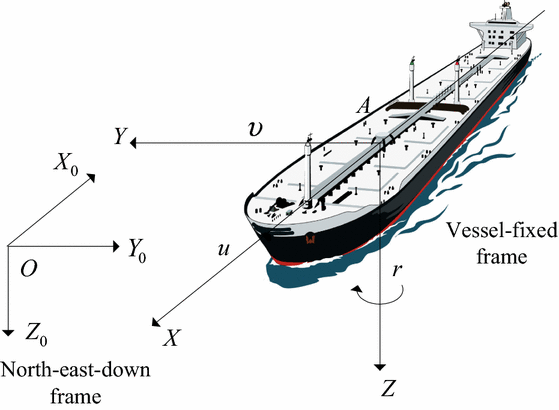
\includegraphics[width=0.55\linewidth]{Pictures/System_Modeling/Reference_Frames_and_Transformations/NED.png}
    \caption{NED coordinate system attached to a marine vehicle. The illustration shows the local navigation axes and their relation to the body frame. Figure taken from a report on robust nonlinear control design for dynamic positioning of marine vessels.\textsuperscript{\cite{NED}}}
    \label{fig:system-modeling-ned-frame}
\end{figure}
\noindent
The relationship between the global and local reference frames follows the transformation chain:
$$
    \text{WGS84 (geodetic)} \;\rightarrow\; \text{ECEF (Cartesian)} \;\rightarrow\; \text{NED (local tangent)} \;\rightarrow\; \text{Body (vehicle-fixed)}
$$
GNSS receivers typically provide positions in the WGS84 frame, expressed as geodetic coordinates $(\varphi, \lambda, h)$, where $\varphi$ is latitude, $\lambda$ is longitude, and $h$ is altitude above the reference ellipsoid. For computational purposes, these coordinates are first converted to the ECEF frame, which represents positions in Cartesian coordinates $(x, y, z)$ relative to the Earth's center of mass.  
\\ \\
To obtain a local navigation frame, the ECEF position is then rotated and translated into the NED frame, which defines a tangent plane fixed at a chosen reference point $(\varphi_0, \lambda_0)$. The rotation from ECEF to NED is given by
$$
    R_{e}^{n} =
    \begin{bmatrix}
        -\sin\varphi_0\cos\lambda_0 & -\sin\varphi_0\sin\lambda_0 & \cos\varphi_0 \\
        -\sin\lambda_0 & \cos\lambda_0 & 0 \\
        -\cos\varphi_0\cos\lambda_0 & -\cos\varphi_0\sin\lambda_0 & -\sin\varphi_0
    \end{bmatrix}
$$
where $\varphi_0$ and $\lambda_0$ are the latitude and longitude of the local origin. The superscript $n$ and subscript $e$ indicate that this matrix transforms a vector expressed in the ECEF frame $\{e\}$ into the NED frame $\{n\}$.  
\\ \\
Given the ECEF position of the vehicle $\mathbf{p}_{b/e}^{e}$ and the ECEF position of the NED origin $\mathbf{p}_{O/e}^{e}$, the vehicles position in NED coordinates is computed as
$$
    \mathbf{p}_{b/O}^{n} = \mathbf{p}_{b/e}^{n} + \mathbf{p}_{e/O}^{n} = R_e^n (\mathbf{p}_{b/e}^{e} - \mathbf{p}_{O/e}^{e})
$$
For onboard sensors, the position of a sensor $\{s\}$ relative to the vehicle body origin, expressed in the NED frame, is given by
$$
\mathbf{p}_{s/b}^{n} = R_b^n \mathbf{p}_{s/b}^{b}
$$
The absolute position of the sensor relative to the NED origin can then be found as
$$
\mathbf{p}_{s/O}^{n} = \mathbf{p}_{s/b}^{n} + \mathbf{p}_{b/O}^{n}
$$
where $\mathbf{p}_{s/b}^{b}$ is the known position of the sensor in the body frame, and $R_b^n$ is the rotation matrix representing the vehicles attitude from the Body to the NED frame.
\\ \\
This formulation relates the sensor position to the global reference frame by first rotating the sensor offset from the body frame into the navigation frame, then translating it using the vehicles global position. The rotation matrix $R_b^n$ is obtained from the vehicles orientation representation, typically parameterized using Euler angles or a unit quaternion, ensuring consistent alignment between the sensor, body, and navigation coordinate frames.
\\ \\
Maintaining a consistent chain of transformations between these frames is essential for reliable navigation and estimation. In practice, GNSS delivers global positions in WGS84 or ECEF coordinates, while onboard IMU sensors provide measurements in the Body frame. Sensor fusion algorithms such as the Extended Kalman Filter (EKF) and Error State Kalman Filter (ESKF) depend on these transformations to express all quantities consistently within the NED frame used for state estimation and control.
